\documentclass{standalone}
%\documentclass[10pt,a4paper]{article} 

% packages
\usepackage{tikz}
\usepackage{pgfplots}
\usetikzlibrary{hobby}
\usetikzlibrary{trees}
\pgfplotsset{compat=1.15}

\usetikzlibrary{calc}
\usepackage{etoolbox}
\usepackage{tikz-network}

% set up layers 
\pgfdeclarelayer{shading}
\pgfdeclarelayer{map}
\pgfdeclarelayer{background}
\pgfdeclarelayer{foreground}
\pgfdeclarelayer{debug}
\pgfdeclarelayer{sankeydebug}
\pgfdeclarelayer{annotate}
\pgfsetlayers{shading,map,background,main,foreground,annotate,sankeydebug,debug}
%

% map
% node tokens
% dependency
% strata
% flows
%   - 
%   - 
% annotations
% debug

% https://tex.stackexchange.com/questions/121286/error-with-hobbyconvexpath
\newcommand{\hobbyconvexpath}[2]{
[   
    create hobbyhullnodes/.code={
        \global\edef\namelist{#1}
        \foreach [count=\counter] \nodename in \namelist {
            \global\edef\numberofnodes{\counter}
            \node at (\nodename)
[draw=none,name=hobbyhullnode\counter] {};
        }
        \node at (hobbyhullnode\numberofnodes)
[name=hobbyhullnode0,draw=none] {};
        \pgfmathtruncatemacro\lastnumber{\numberofnodes+1}
        \node at (hobbyhullnode1)
[name=hobbyhullnode\lastnumber,draw=none] {};
    },
    create hobbyhullnodes
]
($(hobbyhullnode1)!#2!-90:(hobbyhullnode0)$)
\pgfextra{
  \gdef\hullpath{}
\foreach [
    evaluate=\currentnode as \previousnode using int(\currentnode-1),
    evaluate=\currentnode as \nextnode using int(\currentnode+1)
    ] \currentnode in {1,...,\numberofnodes} {
    \ifnum\currentnode=1\relax
    \xdef\hullpath{([closed=true]$(hobbyhullnode\currentnode)!#2!180:(hobbyhullnode\previousnode)$)
  ..($(hobbyhullnode\nextnode)!0.5!(hobbyhullnode\currentnode)$)}
    \else
    \xdef\hullpath{\hullpath
  ..($(hobbyhullnode\currentnode)!#2!180:(hobbyhullnode\previousnode)$)
  ..($(hobbyhullnode\nextnode)!0.5!(hobbyhullnode\currentnode)$)}
    \fi
    \ifx\currentnode\numberofnodes
    \else
    \xdef\hullpath{\hullpath
  ..($(hobbyhullnode\nextnode)!#2!-90:(hobbyhullnode\currentnode)$)}
    \fi
}
}
\hullpath
}

% DEFINE COLOURS 
\definecolor{layer1}{RGB}{208,217,238}
\definecolor{layer2}{RGB}{164,185,225}

%\definecolor{CJBSyellow}{RGB}{249,172,24}

\newif\ifsankeydebug



\begin{document}

    % default units and scale 
    \SetDefaultUnit{cm}
    \SetDistanceScale{1}

    %change aspect ratio as necessary 
    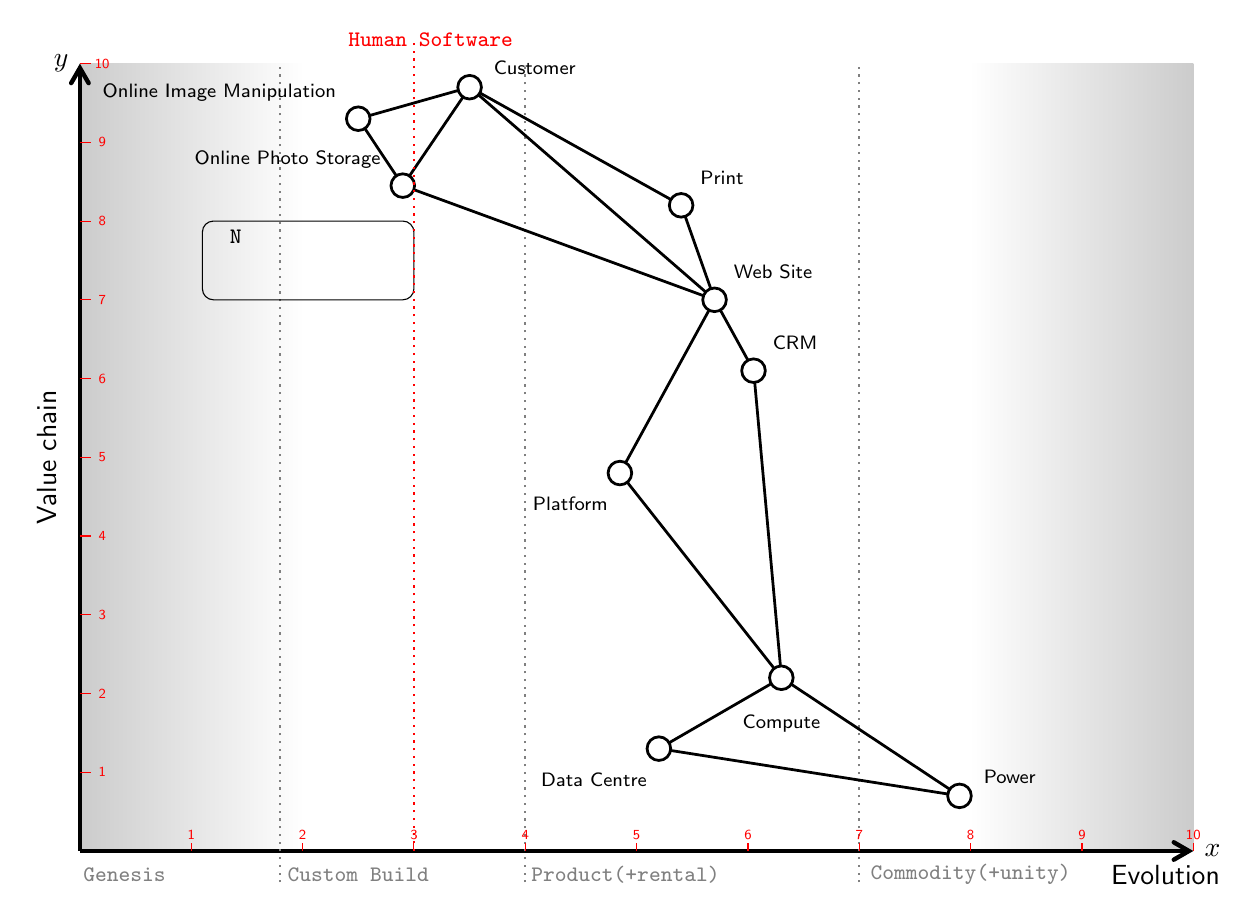
\begin{tikzpicture}[xscale=1.414,yscale=1] 
    
    % only show part of the map, comment out for whole map
    %\clip (5,0) rectangle (10,5);
    
        \sffamily
    
        %%% MAP %%%
        %Mishcon layers defined in Preamble
%color={247,193,152}

%Everything in this TeX file is in the Shading layer
\begin{pgfonlayer}{shading}

%Application Strata
%\fill[color=layer1,opacity=0.5] (0,7.5) rectangle (10,10);
%\node[align=left,rotate=90,color=black!] at (0.3,8.75) {\footnotesize{Applications}};

%Wadley maturity shading
\shade[left color=gray!80,right color=white,opacity=0.5] (0,0) rectangle (2,10);
\shade[left color=white,right color=white,opacity=0.5] (2,0) rectangle (8,10);
\shade[left color=white,right color=gray!80,opacity=0.5] (8,0) rectangle (10,10);


\end{pgfonlayer}
        
\begin{pgfonlayer}{map}

% help lines if useful 
%\draw[help lines, step=0.5, color=gray!30, dashed] (0,0) grid (10,10);
 
% x and y axis    
\draw[->,>=angle 60, ultra thick] (0,0)--(10,0) node[right]{$x$};
\node[align=left] at (9.75,-0.3) {Evolution};
    
\draw[->,>=angle 60, ultra thick] (0,0)--(0,10) node[left]{$y$};
\node[align=left,rotate=90] at (-0.3,5) {Value chain};
    
% Genesis
\Text[x=0.4,y=-0.3,color=gray,fontsize=\footnotesize]{\texttt{Genesis}};

% Custom Build
\draw[-, dotted, color=gray, thick] (1.8,-0.4)--(1.8,10);
\Text[x=2.5,y=-0.3,color=gray,fontsize=\footnotesize]{\texttt{Custom Build}};
     
% Product(+rental)
\draw[-, dotted, color=gray, thick] (4,-0.4)--(4,10);
\Text[x=4.9,y=-0.3,color=gray,fontsize=\footnotesize]{\texttt{Product(+rental)}};
   
% Commodity(+unity)
\draw[-, dotted, color=gray, thick] (7,-0.4)--(7,10);
\Text[x=8,y=-0.3,color=gray,fontsize=\footnotesize]{\texttt{Commodity(+unity)}}

% Numbering / ticks is useful
% Comment out as desired but you can just omitt whole debug layer 
\begin{pgfonlayer}{debug}
% X-AXIS
\draw[-,color=red, thin] (1,0)--(1,0.1);
\Text[x=1,y=0.2,fontsize=\tiny,color=red]{1};
\draw[-,color=red, thin] (2,0)--(2,0.1);
\Text[x=2,y=0.2,fontsize=\tiny,color=red]{2};
\draw[-,color=red, thin] (3,0)--(3,0.1);
\Text[x=3,y=0.2,fontsize=\tiny,color=red]{3};
\draw[-,color=red, thin] (4,0)--(4,0.1);
\Text[x=4,y=0.2,fontsize=\tiny,color=red]{4};
\draw[-,color=red, thin] (5,0)--(5,0.1);
\Text[x=5,y=0.2,fontsize=\tiny,color=red]{5};
\draw[-,color=red, thin] (6,0)--(6,0.1);
\Text[x=6,y=0.2,fontsize=\tiny,color=red]{6};
\draw[-,color=red, thin] (7,0)--(7,0.1);
\Text[x=7,y=0.2,fontsize=\tiny,color=red]{7};
\draw[-,color=red, thin] (8,0)--(8,0.1);
\Text[x=8,y=0.2,fontsize=\tiny,color=red]{8};
\draw[-,color=red, thin] (9,0)--(9,0.1);
\Text[x=9,y=0.2,fontsize=\tiny,color=red]{9};
\draw[-,color=red, thin] (10,0)--(10,0.1);
\Text[x=10,y=0.2,fontsize=\tiny,color=red]{10};
% Y-AXIS
\draw[-,color=red, thin] (0,1)--(0.1,1);
\Text[x=0.2,y=1,fontsize=\tiny,color=red]{1};
\draw[-,color=red, thin] (0,2)--(0.1,2);
\Text[x=0.2,y=2,fontsize=\tiny,color=red]{2};
\draw[-,color=red, thin] (0,3)--(0.1,3);
\Text[x=0.2,y=3,fontsize=\tiny,color=red]{3};
\draw[-,color=red, thin] (0,4)--(0.1,4);
\Text[x=0.2,y=4,fontsize=\tiny,color=red]{4};
\draw[-,color=red, thin] (0,5)--(0.1,5);
\Text[x=0.2,y=5,fontsize=\tiny,color=red]{5};
\draw[-,color=red, thin] (0,6)--(0.1,6);
\Text[x=0.2,y=6,fontsize=\tiny,color=red]{6};
\draw[-,color=red, thin] (0,6)--(0.1,6);
\Text[x=0.2,y=7,fontsize=\tiny,color=red]{7};
\draw[-,color=red, thin] (0,7)--(0.1,7);
\Text[x=0.2,y=8,fontsize=\tiny,color=red]{8};
\draw[-,color=red, thin] (0,8)--(0.1,8);
\Text[x=0.2,y=9,fontsize=\tiny,color=red]{9};
\draw[-,color=red, thin] (0,9)--(0.1,9);
\Text[x=0.2,y=10,fontsize=\tiny,color=red]{10};
\draw[-,color=red, thin] (0,10)--(0.1,10);
\end{pgfonlayer}


\end{pgfonlayer}
        
\tikzset{key/.pic={
    \draw[fill=white](0,0) rectangle (2,2){};
    \Text[x=0.4,y=1.8,color=black,fontsize=\footnotesize]{\texttt{Key:}};
    
    % Practice
    \Vertex[x=0.4,y=1.3,size=0.3,color=black,position=0,distance=1.0,fontcolor=black,shape = diamond,IdAsLabel]{Practise}
    
    % Activity
    \Vertex[x=0.4,y=0.8,size=0.3,color=gray!50,position=0,distance=1.0,fontcolor=black,shape = rectangle,IdAsLabel]{Activity}

    % Resource
    \Vertex[x=0.4,y=0.3,size=0.3,color=white,position=0,distance=1.0,fontcolor=black,shape = circle,IdAsLabel]{Resource}
    
}}

% position Key on Map from bottom left corner
%\path pic () at (1,7.5) {key};



    
        %%% NODES %%% 
        %%%% APPLICATION LAYER VERTICES %%%%%%

% Customer
\Vertex[x=3.5,y=9.7,size=0.3,color=white,position=10,distance=1.0,fontcolor=black,shape=circle,IdAsLabel]{Customer}

% Online Image Manipulation
\Vertex[x=2.5,y=9.3,size=0.3,color=white,position=150,distance=1.0,fontcolor=black,shape=circle,IdAsLabel]{Online Image Manipulation}

% Online Photo Storage
\Vertex[x=2.9,y=8.45,size=0.3,color=white,position=150,distance=1.0,fontcolor=black,shape=circle,IdAsLabel]{Online Photo Storage}

% Print
\Vertex[x=5.4,y=8.2,size=0.3,color=white,position=50,distance=1.0,fontcolor=black,shape=circle,IdAsLabel]{Print}

% Web Site
\Vertex[x=5.7,y=7,size=0.3,color=white,position=50,distance=1.0,fontcolor=black,shape=circle,IdAsLabel]{Web Site}

% CRM
\Vertex[x=6.05,y=6.1,size=0.3,color=white,position=50,distance=1.0,fontcolor=black,shape=circle,IdAsLabel]{CRM}

% Platform
\Vertex[x=4.85,y=4.8,size=0.3,color=white,position=-100,distance=1.0,fontcolor=black,shape=circle,IdAsLabel]{Platform}

% Compute
\Vertex[x=6.3,y=2.2,size=0.3,color=white,position=-90,distance=0.2cm,fontcolor=black,shape=circle,IdAsLabel]{Compute}

% Data Centre
\Vertex[x=5.2,y=1.3,size=0.3,color=white,position=-100,distance=1.0,fontcolor=black,shape=circle,IdAsLabel]{Data Centre}

% Power
\Vertex[x=7.9,y=0.7,size=0.3,color=white,position=10,distance=1.0,fontcolor=black,shape=circle,IdAsLabel]{Power}


        
        %%% PLATES %%% 
        %% Example Plate
\begin{pgfonlayer}{background}
\draw[rounded corners](1.1,7) rectangle (3,8){};
\node[align=left,rotate=0,color=black!] at (1.4,7.8) {\footnotesize{\texttt{N}}};
\end{pgfonlayer}

        
        %%% EDGES %%% 
        %%%% APPLICATION LAYER EDGES %%%%%%

% Customer
\Edge[lw=1.0,color=black,opacity=1,bend=0](Customer)(Online Image Manipulation)
\Edge[lw=1.0,color=black,opacity=1,bend=0](Customer)(Online Photo Storage)
\Edge[lw=1.0,color=black,opacity=1,bend=0](Customer)(Print)
\Edge[lw=1.0,color=black,opacity=1,bend=0](Customer)(Web Site)

% Online Image Manipulation
\Edge[lw=1.0,color=black,opacity=1,bend=0](Online Image Manipulation)(Online Photo Storage)

% Online Photo Storage
\Edge[lw=1.0,color=black,opacity=1,bend=0](Online Photo Storage)(Web Site)

% Print
\Edge[lw=1.0,color=black,opacity=1,bend=0](Print)(Web Site)

% Web Site
\Edge[lw=1.0,color=black,opacity=1,bend=0](Web Site)(CRM)
\Edge[lw=1.0,color=black,opacity=1,bend=0](Web Site)(Platform)

% CRM
\Edge[lw=1.0,color=black,opacity=1,bend=0](CRM)(Compute)

% Platform
\Edge[lw=1.0,color=black,opacity=1,bend=0](Platform)(Compute)

% Compute
\Edge[lw=1.0,color=black,opacity=1,bend=0](Compute)(Data Centre)
\Edge[lw=1.0,color=black,opacity=1,bend=0](Compute)(Power)

% Data Centre
\Edge[lw=1.0,color=black,opacity=1,bend=0](Data Centre)(Power)

% Power
       
        %%% LAYERS %%%
        %%% Human/Software 
\begin{pgfonlayer}{annotate}
\draw[-, dotted, color=red, thick] (3,0)--(3,10.3);
\Text[x=3.15,y=10.3,color=red,fontsize=\footnotesize]{\texttt{Human Software}};
\end{pgfonlayer}{annotate}


        
        %


        %\input{layers/StrategyLayerE.tex}
        
        
        

    \end{tikzpicture}

   
    
\end{document}


